% The ACM Web Conference 2027, Research Track, Semantics and Knowledge.
% https://www2027.thewebconf.org/research-track-papers/
% Submission format: \documentclass[sigconf, review, anonymous]{acmart};
% at most 8 pages of content plus up to 4 pages of references and appendix.
\documentclass[sigconf, review, anonymous]{acmart}
% \documentclass[sigconf]{acmart} % camera-ready

% acmart already loads amsmath, booktabs, graphicx, and newtxmath;
% do not load amssymb, which clashes with newtxmath.
\usepackage{multirow}
\usepackage{array}
\usepackage{pifont}
\usepackage{booktabs,tabularx,array}
\usepackage{xcolor}
\usepackage{colortbl}
\newcolumntype{C}[1]{>{\centering\arraybackslash}p{#1}} % fixed-width centred column for results tables
\setlength{\emergencystretch}{2em} % fewer overfull lines with long system names

\usepackage{todonotes}
% \usepackage[disable]{todonotes}
\newcommand{\oshani}[1]{\todo[inline, color=blue!40, author=\textbf{Oshani}]{#1}}
\newcommand{\maruf}[1]{\todo[inline, color=red!40, author=\textbf{Maruf}]{#1}}
\newcommand{\abid}[1]{\todo[inline, color=green!40, author=\textbf{Abid}]{#1}}

\settopmatter{printacmref=false}
\setcopyright{none}
\renewcommand\footnotetextcopyrightpermission[1]{}

% ---------------------------------------------------------------------------
% Notation. \sys is the system name everywhere in the text; change it in one
% place. \tbd marks a result cell that is filled after the UNH runs finish.
% ---------------------------------------------------------------------------
\newcommand{\sys}{UNH}
\newcommand{\sysfull}{Unified Narrative Hypergraph}
\newcommand{\tbd}{--}
\providecommand{\argmax}{\operatorname*{arg\,max}}
\newcommand{\rel}[1]{\textsc{#1}}            % relation label, e.g. \rel{causes}
\newcommand{\Ecf}{E_{CF}}
\newcommand{\Efv}{E_{FV}}
\newcommand{\Eff}{E_{FF}}
\newcommand{\simcos}{\operatorname{cos}}
% feature table marks
\newcommand{\yes}{\ding{51}}
\newcommand{\no}{\ding{55}}
\newcommand{\half}{$\circ$}
\newcommand{\na}{--}
% figure that compiles before its file exists
\newcommand{\figorbox}[3]{\IfFileExists{#1}{\includegraphics[width=#2]{#1}}{\fbox{\parbox[c][#3][c]{0.95#2}{\centering\small Placeholder: \texttt{\detokenize{#1}}}}}}

\begin{document}

\title{UNH: A Unified Narrative Hypergraph for Dependency-Aware Retrieval}

\author{Abid Talukder}
\affiliation{%
  \institution{Rensselaer Polytechnic Institute}
  \city{Troy}
  \state{New York}
  \country{USA}}
\email{taluka@rpi.edu}

\author{Maruf Ahmed Mridul}
\affiliation{%
  \institution{Rensselaer Polytechnic Institute}
  \city{Troy}
  \state{New York}
  \country{USA}}
\email{mridum@rpi.edu}

\author{Oshani Seneviratne}
\affiliation{%
  \institution{Rensselaer Polytechnic Institute}
  \city{Troy}
  \state{New York}
  \country{USA}}
\email{senevo@rpi.edu}

\renewcommand{\shortauthors}{Talukder et al.}


\begin{abstract}
Answering questions over complex documents often requires
connecting dispersed statements and their dependencies,
such as exceptions, prerequisites, and conditional
consequences. Existing structured retrieval methods
capture complementary aspects of document knowledge,
including entity participation and semantic relationships
between statements. We introduce the \emph{\sysfull} (\sys{}), a persistent, source-linked index that
integrates these forms of connectivity. Each fact is both
a hyperedge over its participants and a node in a graph
of typed inter-fact dependencies. During indexing, UNH
proposes candidate dependencies by matching questions
one fact raises with those another answers, alongside
textual and contextual similarity. At query time, it
assembles connected evidence without retrieval-time
LLM calls, optionally supplemented with source passages.
We evaluate UNH on HotpotQA, MuSiQue, G-Medical, and a
new QA collection over five long-form insurance documents.
On HotpotQA and MuSiQue, base UNH improves upon the
strongest compact-context baseline, HippoRAG 2, on F1
and LLM-Acc, while approaching HyperGraphRAG with
93--94\% fewer reader-context tokens. Connectivity
ablations show that combining participation and semantic
edges improves judged answer scores over either
restricted view across all four datasets, although
participation-only retrieval achieves slightly higher
Wikipedia F1. Supplementing structured paths with
source passages improves contract QA, particularly
multihop questions, achieving a 92.4 overall judge score
with approximately 74\% fewer reader-context tokens
than HyperGraphRAG, which scores 92.1. On G-Medical,
passage augmentation improves contextual summarization
and generation, while stronger baselines retain higher
overall scores. These findings characterize the
complementary roles of structured connectivity and
source context in evidence retrieval.
\end{abstract}



% \begin{abstract}
% Answering questions over complex documents often requires connecting dispersed statements and their dependencies, such as exceptions, prerequisites, and conditional consequences. Entity-based connections alone may miss these dependencies and the evidence needed to resolve them.
% We introduce the \emph{\sysfull} (\sys{}), a persistent,
% source-linked index in which each fact is both a hyperedge over its participants
% and a node in a graph of typed inter-fact dependencies. During indexing, \sys{} discovers candidate dependencies
% by matching questions one fact raises with those another
% answers, alongside textual and contextual similarity.
% At query time, it assembles connected evidence without
% retrieval-time LLM calls, optionally supplemented with
% source passages.
% We evaluate on HotpotQA, MuSiQue, G-Medical, and a new QA collection over five long-form insurance documents. On HotpotQA and MuSiQue, base \sys{} improves upon the strongest compact-context baseline, HippoRAG 2, on F1 and LLM-Acc, while approaching HyperGraphRAG with 93–94\% fewer reader-context tokens. Adding source passages improves contract QA, particularly multihop questions, achieving a 92.4 overall judge score with approximately 74\% fewer reader-context tokens than HyperGraphRAG, which scores 92.1. Connectivity ablations show that jointly using participation and semantic edges improves judged answer scores over either restricted view across all four datasets, although participation-only retrieval achieves slightly higher Wikipedia F1. On G-Medical, passage augmentation improves contextual summarization and generation, while stronger baselines retain higher overall scores.
% \end{abstract}







\begin{CCSXML}
<ccs2012>
   <concept>
       <concept_id>10002951.10003317.10003338</concept_id>
       <concept_desc>Information systems~Retrieval models and ranking</concept_desc>
       <concept_significance>500</concept_significance>
   </concept>
   <concept>
       <concept_id>10010147.10010178.10010187</concept_id>
       <concept_desc>Computing methodologies~Knowledge representation and reasoning</concept_desc>
       <concept_significance>500</concept_significance>
   </concept>
   <concept>
       <concept_id>10010147.10010178.10010179.10003352</concept_id>
       <concept_desc>Computing methodologies~Information extraction</concept_desc>
       <concept_significance>300</concept_significance>
   </concept>
</ccs2012>
\end{CCSXML}

\ccsdesc[500]{Information systems~Retrieval models and ranking}
\ccsdesc[500]{Computing methodologies~Knowledge representation and reasoning}
\ccsdesc[300]{Computing methodologies~Information extraction}

\keywords{Retrieval-augmented generation, knowledge representation, hypergraphs, discourse relations, fact dependencies, multi-hop question answering, long-document question answering, knowledge graph construction, provenance.}

\maketitle


\abid{Abstract can be made shorter and we don't need to write specific low level results here. We can write something like achieves SOTA with far less tokens.}

\section{Introduction}
\label{sec:introduction}

Answering questions over natural-language documents requires recovering relevant statements and the dependencies governing their interpretation. Rules have exceptions, consequences depend on conditions, and events acquire meaning through context. Evidence may be dispersed across passages and expressed in specialized terminology. Retrieval-augmented generation (RAG) supplies evidence for answer generation~\cite{lewis2020retrieval}, while graph-based RAG organizes knowledge into connected structures~\cite{peng2025graph,han2024retrieval}. The retrieval challenge is to recover both the relevant statements and the connections that determine how they should be interpreted: finding statements about the right entities can leave essential evidence missing. For knowledge-grounded access to Web document collections, this motivates reusable, source-linked semantic indexes that make contextual dependencies available to people and LLM-based agents.

\begin{figure}[t]
    \centering
    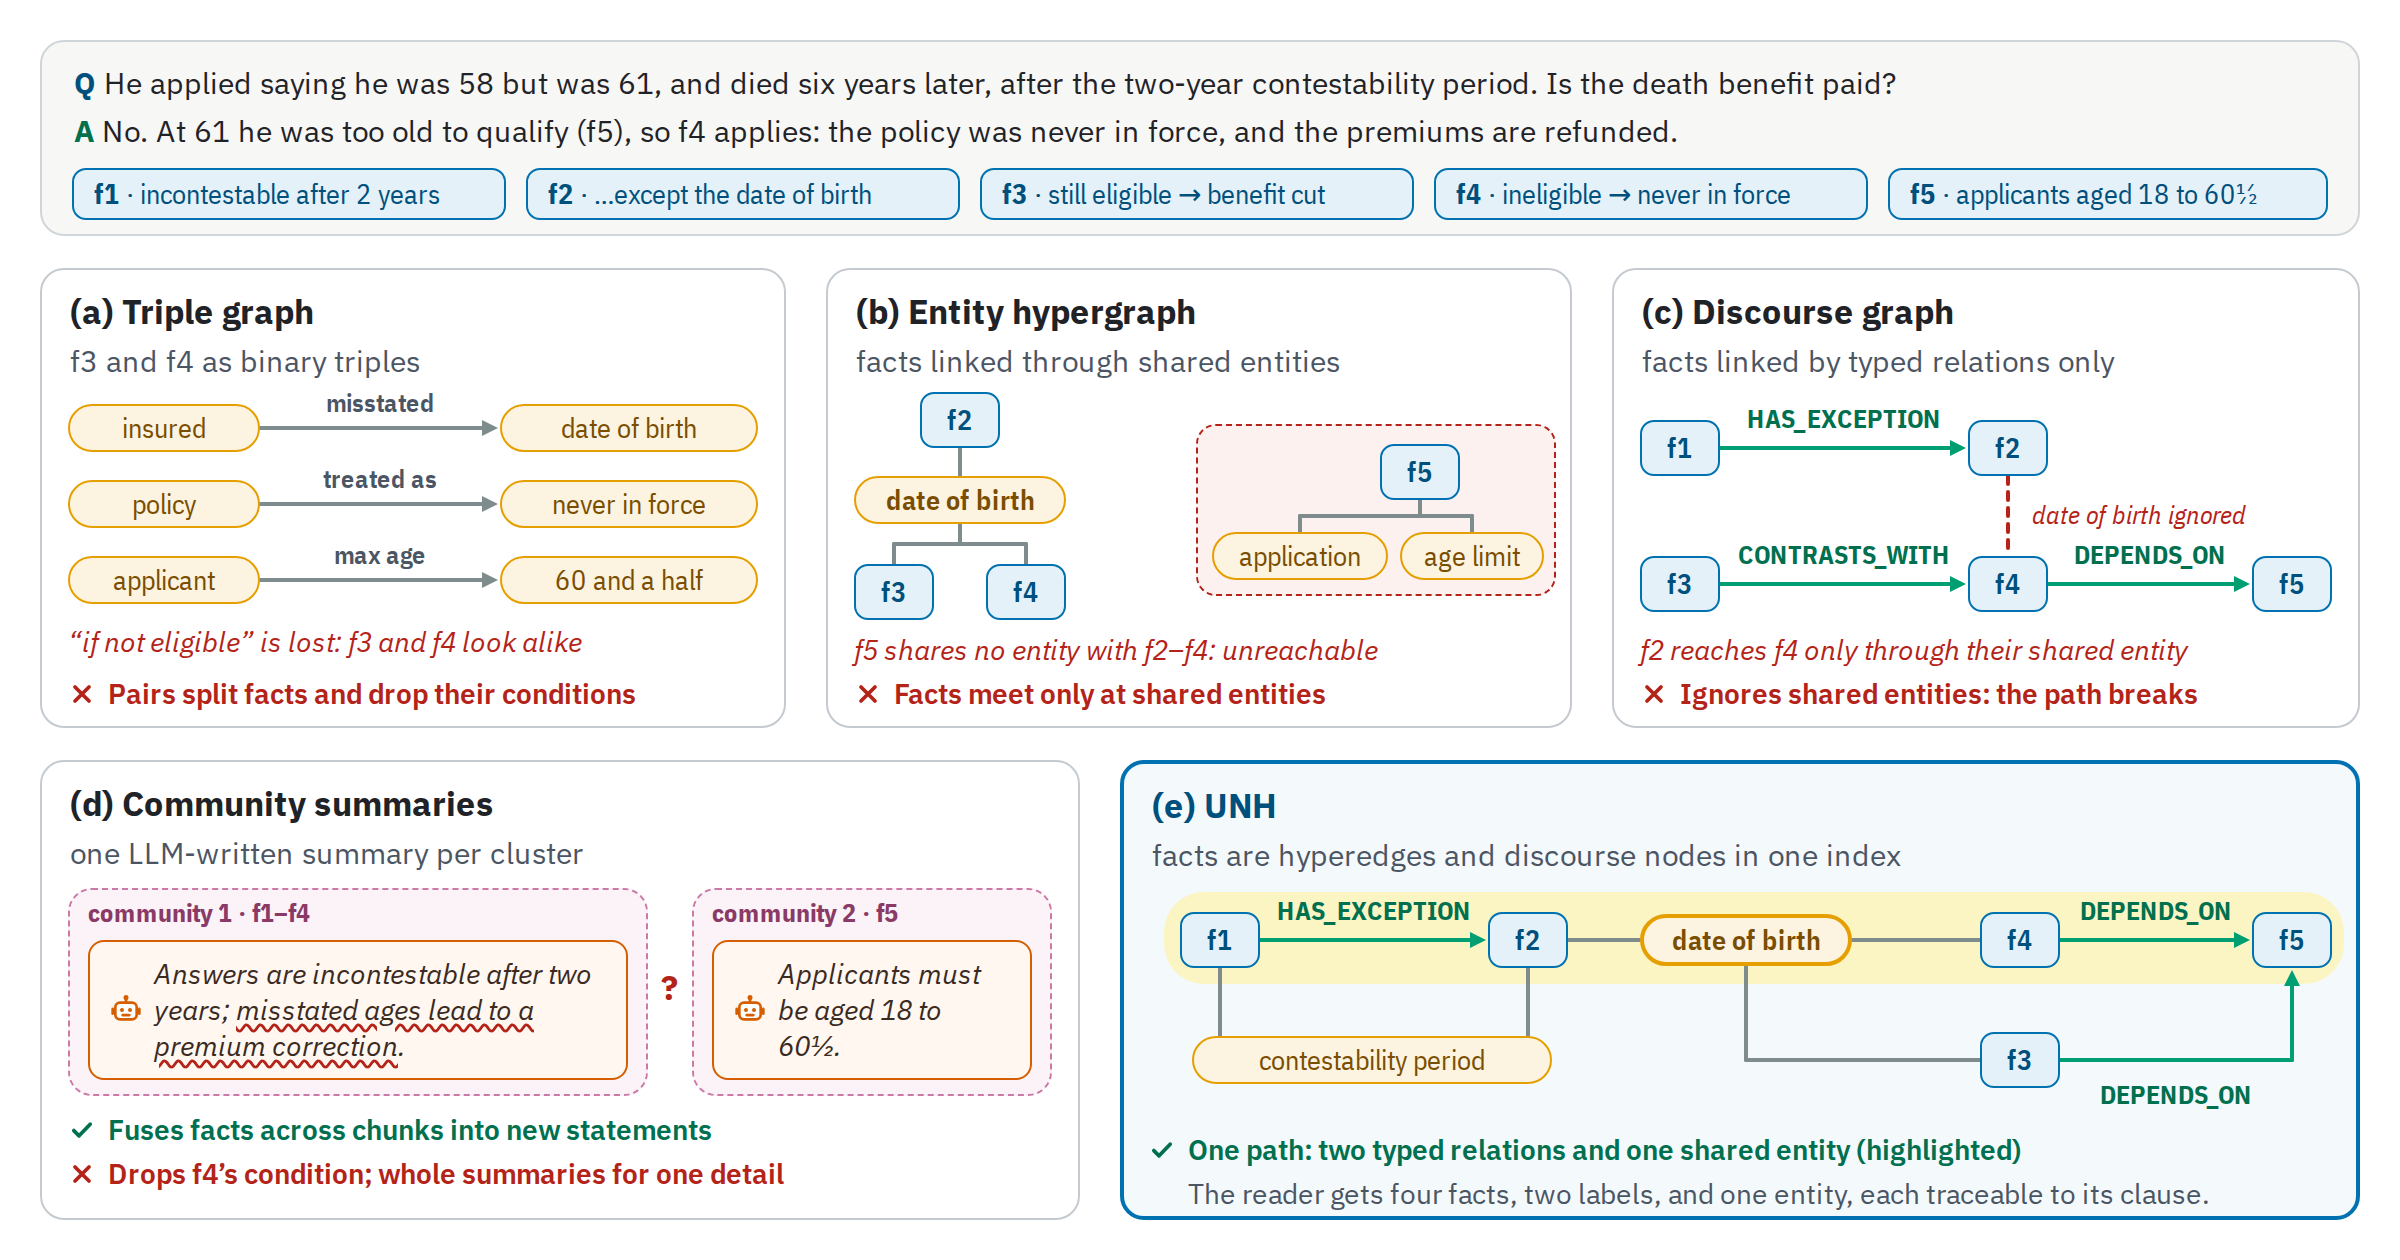
\includegraphics[width=0.9\linewidth]{figures/motivation.png}
    \caption{\normalfont \textbf{Illustrative evidence chain across dispersed provisions.}
    Shared-participant links connect facts, while typed dependencies
    reveal their interactions and help retrieve missing evidence.}
    \label{fig:motivation}
\end{figure}

\abid{For the example shown, it demonstrates well why dependencies between facts need to exist, but it doesn't address why we need BOTH entity and discourse (fact to fact) edges at the same time. Figure 1 question can be solved with the chain alone and no entity relationships. We also need to address why hierarchical summaries that consolidate context can't retrieve this context.}

Consider the question in Figure~\ref{fig:motivation}: \emph{An insured reported an age of 58 but was 61 at application, and died six years later, after the contestability period. Is the death benefit payable?} Under the illustrated policy, answering requires four dispersed provisions: the general contestability rule, its age-misstatement exception, the consequences of a misstatement, and eligibility at the correct age. Retrieving the general rule alone can miss the exception; retrieving the exception without the eligibility provision can leave its consequence unresolved. The required evidence forms a chain in which one provision qualifies another and a separate provision resolves the outcome's condition. The figure illustrates incomplete retrieval that finds the first three provisions but omits the eligibility criterion. This example motivates preserving propositions with their conditions and connecting them to the evidence needed to interpret them.

Existing methods provide complementary capabilities: entity graphs connect entities and relations~\cite{edge2024local,gutierrez2025rag}; hypergraphs and proposition representations preserve joint facts~\cite{luo2025hypergraphrag,wang2025proprag}; event and discourse structures model semantic dependencies~\cite{yang2025eventrag,liu2026discorag}; hierarchical summaries consolidate context~\cite{sarthi2024raptor,zhong2026hygrag}; and query-specific structures organize retrieval around subproblems~\cite{chen2026logicrag}. We introduce the \emph{\sysfull} (\sys{}), which integrates joint fact participation and typed inter-fact dependencies. Rather than treating these as separate representations, \sys{} makes each fact both a hyperedge over its participants and a node connected to other facts through semantic relations. This unified structure supports evidence navigation through both shared entities and inferred dependencies, including connections between facts without shared participants. Table~\ref{tab:positioning} compares these design dimensions.

During indexing, \sys{} proposes candidate dependencies by matching questions one fact raises with those another answers, alongside textual and contextual similarity. Retrieval adapts HippoRAG~2-style graph propagation~\cite{gutierrez2025rag} and assembles paths over participation and dependency links without generative LLM calls. Source passages can supplement these paths before a separate reader generates the answer. We evaluate on HotpotQA~\cite{yang2018hotpotqa}, MuSiQue~\cite{trivedi2022musique}, G-Medical~\cite{xiang2025when}, and a new QA collection over five insurance documents, examining answer quality, reader-context size, construction requirements, connectivity restrictions, and passage augmentation.

Our contributions are:
\begin{itemize}
    \item A unified, source-linked representation of $n$-ary
    participation and typed inter-fact dependencies, enabling
    evidence chains beyond shared-entity connections.

    \item A construction and retrieval framework combining
    question-guided dependency discovery with joint use of
    hypergraph and discourse connectivity for LLM-free
    evidence retrieval.

    \item An evaluation across complementary QA demands,
    characterizing answer quality and reader-context
    trade-offs, the complementary roles of participation
    and semantic connectivity, and the value of
    supplementing structured evidence paths with source
    passages.
\end{itemize}



\section{Related Work}
\label{sec:related_work}

Web knowledge systems preserve statement identity, arguments, qualifications, and provenance through W3C $n$-ary relation instances~\cite{noy2006nary}, Wikidata qualifiers and references~\cite{vrandecic2014wikidata}, RDF-star annotations~\cite{hartig2017rdfstar}, and nanopublications linking assertions to provenance and publication information~\cite{groth2010nanopub}. Automatic index construction draws on LLM-based knowledge extraction and integration~\cite{bian2025llm}, including extraction, definition, and canonicalization in EDC~\cite{zhang2024extract}, entity clustering in KGGen~\cite{mo2025kggen}, and incremental integration in iText2KG~\cite{lairgi2024itext2kg}.
\abid{KGGEN didn't lay the foundation for entity clustering and deduplication (its fairly standard). Possibly we can take about existing event driven structures like Wikievents or other big projects that may be relevant and say that UNH can be used to build these things automatically with provenance?}

Graph-based retrieval uses community reports in Microsoft GraphRAG~\cite{edge2024local}, low- and high-level retrieval in LightRAG~\cite{guo2024lightrag}, and Personalized PageRank in HippoRAG~\cite{gutierrez2024hipporag}. HippoRAG~2 adds passage nodes and query-to-triple linking~\cite{gutierrez2025rag}; MemGraphRAG uses shared schema, fact, and passage memory~\cite{wu2026memgraphrag}. Structured-path reasoning~\cite{sun2023think,ma2024think,luo2023reasoning} and learned graph retrieval~\cite{mavromatis2024gnn} provide additional mechanisms for consuming graph knowledge. Comparative studies show that effectiveness depends on task and design~\cite{zhou2025indepth,xiang2025when}. \sys{} builds on HippoRAG~2-style propagation, but ranks propositions connected through participation and dependency links and assembles evidence paths over those units.

Fact-preserving approaches include $n$-ary hyperedges in HyperGraphRAG~\cite{luo2025hypergraphrag}, hypergraph reasoning in HyperRAG~\cite{lien2026hyperrag}, query-specific hyper-relational graphs in HOLMES~\cite{panda2024holmes}, and thematic and entity hypergraphs in Cog-RAG~\cite{hu2026cograg}. Proposition retrieval~\cite{chen2024dense}, atomic-fact evaluation~\cite{min2023factscore}, and agentic exploration of atomic facts~\cite{li2024graphreader} likewise motivate preserving statements as evidence units. PropRAG retains proposition-level entity co-occurrence as implicit hyperedges and retrieves proposition paths through LLM-free beam search~\cite{wang2025proprag}. SiReRAG indexes similar and entity-related information~\cite{zhang2025sirerag}, while AtomicRAG and ToPG organize atom--entity and proposition graphs~\cite{hou2026atomicrag,delmas2026topg}. \sys{} supplements participant connectivity with explicit inter-fact relations, whose edges provide traversal routes and whose labels describe inferred dependencies to the reader.

Dependency modeling draws on discourse relations~\cite{mann1988rhetorical,prasad2017penn}, eventuality graphs~\cite{zhang2020aser}, and event-centric multihop QA beyond entity bridges~\cite{li2024meqa}. EventRAG connects events through logical and temporal relations and uses iterative agent-based retrieval~\cite{yang2025eventrag}; related approaches exploit causal graphs~\cite{wang2025causalrag}, entity--event context~\cite{zhang2026e2rag}, and temporally grounded event units~\cite{sun2025dygrag}. Disco-RAG combines offline intra-chunk discourse trees with an inter-chunk rhetorical graph constructed at query time over retrieved evidence~\cite{liu2026discorag}. \sys{} instead constructs cross-passage dependencies during indexing, making them available to retrieve additional statements alongside participation links.

Other approaches consolidate evidence through recursive summaries~\cite{sarthi2024raptor}, heterogeneous information units~\cite{xu2025noderag}, hierarchical contextual and relational summaries~\cite{zhong2026hygrag}, linked memories~\cite{xu2025amem}, and global memory~\cite{qian2024memorag}. Dependencies may be expressed in their generated text; explicit edges additionally expose individual connections for traversal. Query-time methods interleave reasoning and retrieval~\cite{trivedi2023interleaving}, plan retrieval~\cite{verma2025planrag}, or construct adaptive reasoning structures without a prebuilt corpus graph~\cite{chen2026logicrag}.
\abid{This explains breadth of existing approaches well, but it doesn't address gaps in existing approaches. For example, in the fact preserving n-ary, UNH says it supplements with explicit inter-fact relations and for discourse (inter-fact) relation graphs it adds participant entity edges. Why doesn't each one work alone? In which situation might they break? Most importantly, why do you need both to co-exist at the same time during retrieval? How does UNH solve this situation and close the gap?}

Table~\ref{tab:positioning} summarizes these design distinctions. \sys{} integrates joint-participant facts, question-guided cross-passage dependency discovery, and source provenance in a persistent index. Retrieval combines participation and semantic connectivity through graph propagation and evidence-path assembly without retrieval-time LLM calls. The connectivity ablations assess the use of these two structures within the same extracted index.



\abid{We need to edit table 1 on design level comparisons. Dependency aware retrieval is slightly confusing and very broad. Technically, any graph thats answering a question has dependencies between information encoded? Also, LOGICRAG does use dependencies since it creates a DAG of subproblems and which subproblems are dependent on the context of a previous subproblem.}
\begin{table}[t]
\centering
\caption{\normalfont \textbf{Design-level comparison of structured RAG methods, based on each method’s described mechanism rather than measured performance.}
$\checkmark$: explicit; $\circ$: qualified;
$\times$: absent from the described mechanism; ---: not applicable.}
\label{tab:positioning}
\scriptsize
\setlength{\tabcolsep}{2pt}
\renewcommand{\arraystretch}{1.15}

\begin{tabularx}{\columnwidth}
{@{}l*{6}{>{\centering\arraybackslash}X}@{}}
\toprule
& \multicolumn{3}{c}{Representation}
& \multicolumn{2}{c}{Utilization}
& Efficiency \\
\cmidrule(lr){2-4}
\cmidrule(lr){5-6}
\cmidrule(l){7-7}
Method
& \shortstack{Joint\\$n$-ary\\facts}
& \shortstack{Typed\\fact\\relations}
& \shortstack{Links\\without\\shared\\entities}
& \shortstack{Dependency-\\aware\\retrieval}
& \shortstack{Source\\links}
& \shortstack{$\leq 1$ online\\LLM call} \\
\midrule
MS GraphRAG (local)~\cite{edge2024local}
& $\times$ & $\times$ & $\times$
& $\times$ & $\checkmark$ & $\checkmark$ \\

HippoRAG 2~\cite{gutierrez2025rag}
& $\times$ & $\times$ & $\times$
& $\times$ & $\checkmark$ & $\checkmark$ \\

MemGraphRAG~\cite{wu2026memgraphrag}
& $\times$ & $\times$ & $\times$
& $\times$ & $\checkmark$ & $\checkmark$ \\

HyperGraphRAG~\cite{luo2025hypergraphrag}
& $\checkmark$ & $\times$ & $\times$
& $\times$ & $\checkmark$ & $\checkmark$ \\

PropRAG~\cite{wang2025proprag}
& $\checkmark$ & $\times$ & $\times$
& $\times$ & $\checkmark$ & $\checkmark$ \\

HyGRAG~\cite{zhong2026hygrag}
& $\times$ & $\times$ & $\times$
& $\times$ & $\checkmark$ & $\checkmark$ \\

EventRAG~\cite{yang2025eventrag}
& $\checkmark$ & $\checkmark$ & $\checkmark$
& $\checkmark$ & $\circ$ & $\times$ \\

Disco-RAG~\cite{liu2026discorag}
& $\times$ & $\circ$ & $\circ$
& $\times$ & $\checkmark$ & $\times$ \\

LogicRAG~\cite{chen2026logicrag}
& --- & --- & ---
& $\circ$ & $\circ$ & $\times$ \\
\midrule
\textbf{\sys{} (ours)}
& $\checkmark$ & $\checkmark$ & $\checkmark$
& $\checkmark$ & $\checkmark$ & $\checkmark$ \\
\bottomrule
\end{tabularx}

\smallskip
\begin{minipage}{\columnwidth}
\scriptsize
\textit{Scope.}
Fact relations and entity-independent links connect statements or events.
Dependency-aware retrieval uses these connections to select further evidence.
Source links denote passage mappings ($\checkmark$) or source-derived context
and entry provenance ($\circ$). Online LLM counts exclude indexing and final
answer generation.

\textit{Qualifications.}
Disco-RAG models discourse units and chunks after retrieval.
LogicRAG uses subquestion dependencies and rolling summaries.
EventRAG preserves entry provenance during fusion and permits LLM-based
knowledge expansion.
\end{minipage}
\end{table}














\section{Methodology}
\label{sec:method}

\sys{} retrieves evidence from a document corpus $\mathcal{D}$ by combining
entity participation in facts with semantic relations between facts. The two
structures support complementary retrieval steps: shared participants connect
statements about the same entity, while semantic relations connect statements
through dependencies, exceptions, causality, or other relationships. We first
construct this unified index offline, then retrieve and rank evidence chains
for each question $q$. A separate reader LLM answers from the selected chains. The index preserves
propositions with their conditions, while the retrieved chains expose both
shared participants and inferred dependencies among those propositions.

\subsection{Unified Knowledge Representation}
\label{sec:index}



\begin{figure}[t]
    \centering
    \includegraphics[width=0.8\columnwidth]{figures/graph.pdf}
    \caption{\normalfont  A \sys{} index example showing how shared entities and semantic relations connect facts across sections to determine the outcome of an age misstatement.}
    \label{graph.pdf}
\end{figure}


The index has three node types and three edge types:
$\mathcal{G}=(C,F,V,E_{CF},E_{FV},E_{FF})$, 
where $C$ contains source chunks, $F$ contains facts, and $V$ contains
entities. Each chunk stores its text and a one-sentence summary. Each fact
$f=(s_f,T_f,A_f,U_f)$ stores a self-contained proposition $s_f$, topics
$T_f$, questions it answers $A_f$, and follow-up questions it raises $U_f$.
An entity $v=(n_v,\rho_v)$ stores a canonical name $n_v$ and a
\emph{micro-role} $\rho_v$, a short description of what it denotes or does
in its passage. For example, the micro-role of \emph{date of birth} describes
its use in determining the insured person's age for eligibility and premiums.

Provenance edges $E_{CF}\subseteq C\times F$ associate facts with their
source chunks. Participation edges $E_{FV}\subseteq F\times V$ connect
each fact to its participants. Their set
$V(f)=\{v:(f,v)\in E_{FV}\}$ forms a hyperedge indexed by $f$, retaining
all participants of one proposition together rather than decomposing it into
binary statements. Different facts remain distinct hyperedges even when their
participant sets coincide. Semantic edges
$(f_i,f_j,\ell,r)\in E_{FF}$ connect propositions with a directional label
$\ell$ and an LLM-assigned strength $r\in[0,1]$. Each extracted relation
has a corresponding inverse edge, such as \texttt{exception\_to} and
\texttt{has\_exception}. The edge stores the label and strength; the substantive claims remain in the
endpoint sentences. Strength is an LLM-assigned retrieval signal, not a
calibrated probability or a guarantee of entailment. Participation edges group
entities belonging to one fact; their argument roles and the fact's conditions
remain expressed in the proposition text.

Facts therefore function both as hyperedges over entities and as nodes in a
narrative or discourse graph. The participation structure retains the
participants of a fact, while the semantic structure records how that fact
relates to other propositions, including those without a shared participant.
The two views correspond to hypergraph and discourse-based
representations~\cite{luo2025hypergraphrag,prasad2017penn}.
Their integration enables a retrieval path to alternate between the two
structures, potentially connecting facts that are disconnected in either
restricted view. Our ablations assess the effect of restricting participation
or semantic connectivity during propagation and path
construction while retaining the same extracted index.


\autoref{graph.pdf} illustrates how the two structures complement
each other; it is not a measured retrieval trace. An insured reported
an age of 58 but was 61 at application and died six years later.
Although the contestability period has passed, $f_2$ exempts
date-of-birth misstatements from rule $f_1$. The age limit $f_5$
establishes ineligibility at 61, so $f_4$ applies rather than $f_3$:
no death benefit is payable, and premiums are refunded.
The evidence path
$f_1\to f_2\to\emph{date of birth}\to f_4\to f_5$
requires both structures: participation alone cannot reach $f_5$,
while semantic relations alone cannot connect $f_2$ to $f_4$.


Relevance propagation includes facts, entities, and source
chunks; evidence paths contain only facts and entities. The reader receives fact sentences, entity names and
micro-roles, and the labels connecting them. The remaining fields support
construction or retrieval: chunk summaries contextualize relation extraction,
topics guide candidate dependency discovery, and question annotations
identify complementary facts during construction. They are not added to the
reader's context.

\subsection{Index Construction}
\label{sec:construction}

\begin{figure*}[t]
\centering
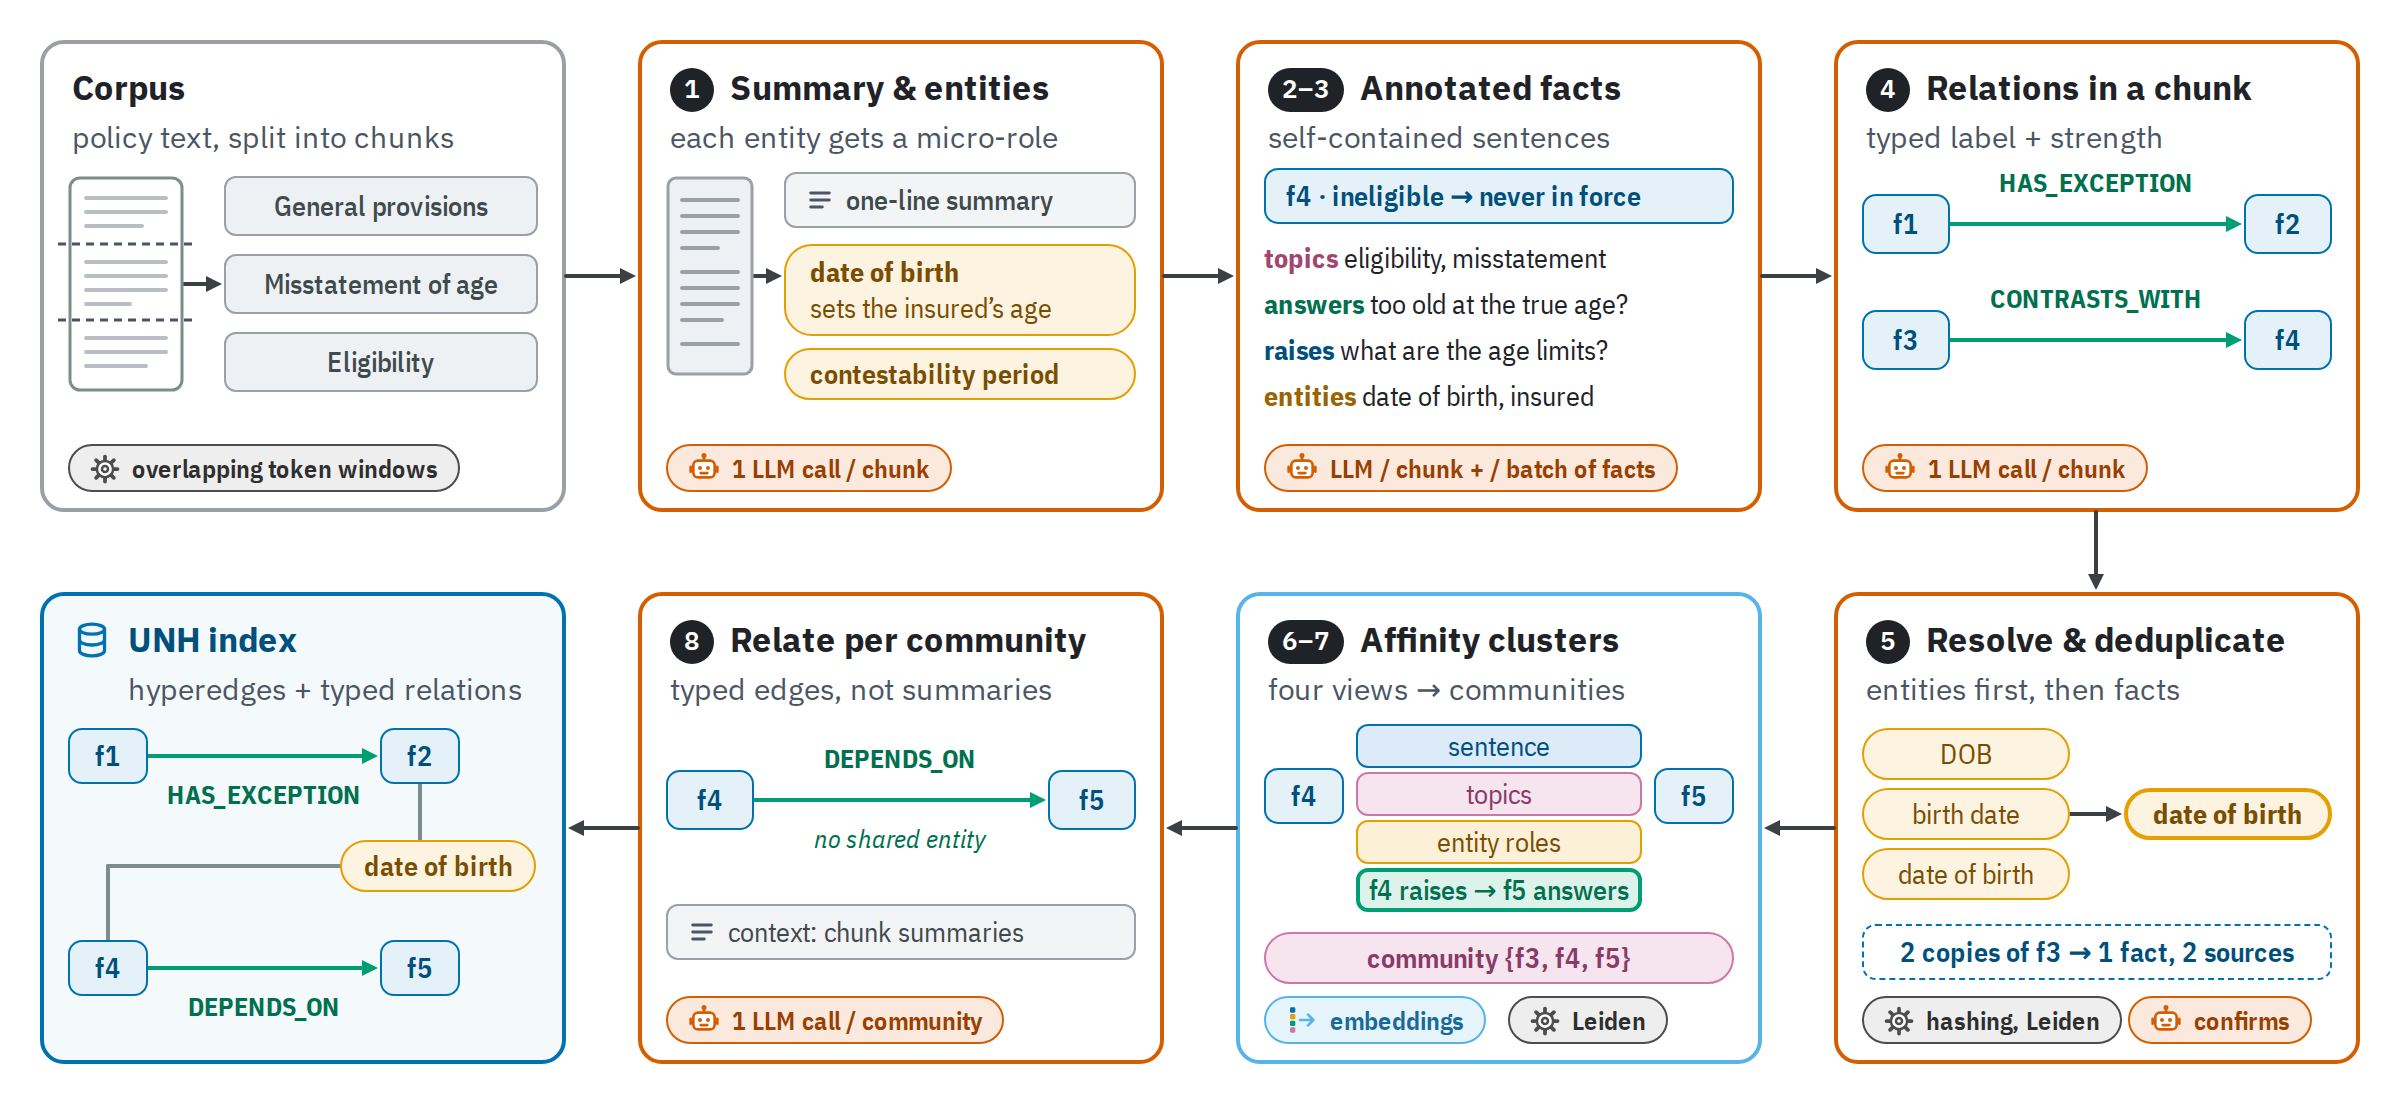
\includegraphics[width=0.8\textwidth]{figures/construction.png}
\caption{Overview of \sys{} index construction.}
\label{fig:construction}
\end{figure*}

Figure~\ref{fig:construction} summarizes index construction. Construction begins with independent extraction from each chunk, followed by
integration of the resulting subgraphs into a corpus-wide index. Short passages, as in HotpotQA~\cite{yang2018hotpotqa} and
MuSiQue~\cite{trivedi2022musique},
are treated as individual chunks prefixed with their titles. The G-Medical corpus~\cite{xiang2025when} and long-form contracts are split
into overlapping token windows.
Every extraction call returns a typed record without
chain-of-thought~\cite{khattab2024dspy}.


For each chunk, an LLM first produces a one-sentence summary and an entity
inventory with canonical names and micro-roles, resolving pronouns and aliases.
A second call extracts atomic, self-contained propositions grounded in the
chunk. Each proposition expresses one claim, event, rule, or state, with
references resolved and conditions retained~\cite{chen2024dense,min2023factscore}.
Separating the two branches of the age-misstatement clause into $f_3$ and
$f_4$, for instance, allows each to receive its own dependency on the
eligibility rule and to be retrieved without unrelated surrounding clauses.

The extracted facts are annotated in batches. Each call receives the chunk,
a batch of facts, and the inventory names, and returns the topics, answered
questions, follow-up questions, and participants of each fact. Participants
are selected from the inventory so that facts refer to shared entity objects.
A returned name is matched exactly to the inventory or, if no exact match
exists, to the closest inventory name under character $n$-gram TF--IDF~\cite{salton1988term}.
Each match creates a participation edge. Answered and follow-up questions describe what a fact settles
and what it leaves open, respectively. This distinction helps
identify relations across sections and documents: $f_4$ explains
the consequence of ineligibility but leaves open how old is too
old, whereas $f_5$ supplies the age limit. These annotations provide candidate-discovery signals for complementary
facts whose wording or participants may differ. The subsequent relation
extraction call determines whether a dependency should be added. 

For each chunk with at least three facts, one call receives
the chunk summary and numbered fact sentences and is asked to identify
related pairs with a forward label, its inverse, and a
strength in $[0,1]$. Labels must describe relations between
propositions, such as \texttt{causes}, \texttt{precedes},
\texttt{exception\_to}, or \texttt{contradicts}, rather than
attributes such as \texttt{has\_amount}. The backward label
must express the inverse relation, as in
\texttt{exception\_to}/\texttt{has\_exception}; zero-strength
pairs are discarded. In the policy example, this step extracts
$f_1$ \texttt{has\_exception} $f_2$ and
$f_3$ \texttt{contrasts\_with} $f_4$.
Each edge stores only its label and strength: the endpoint
facts already contain the substantive information, while the edge makes the connection available to retrieval
and its label identifies the relation in the serialized evidence.

The chunk subgraphs are then merged and duplicate entities resolved through
passes of increasing cost. The first uses exact matching after Unicode NFKC
normalization, lower-casing, and singularization; the second uses semantic
hashing at high similarity with SemHash.\footnote{\url{https://github.com/MinishLab/semhash}.}
Remaining candidates form a nearest-neighbour graph that weights name
similarity more strongly than micro-role similarity. Leiden
clustering~\cite{traag2019leiden} partitions the graph, and small clusters
are packed for LLM processing. Each call identifies equivalent entities and
assigns canonical names and micro-roles, after which participation edges are
redirected to the canonical nodes. Micro-roles provide contextual evidence for the final equivalence decisions.
The earlier name-based passes are heuristic and do not establish contextual
identity; errors introduced there can affect subsequent connectivity. In the policy
example, resolving references to \emph{date of birth} across
sections creates the shared entity through which retrieval
moves from the exception $f_2$ to the misstatement clause $f_4$. Fact consolidation uses an analogous fact-similarity
graph to group candidate repeated propositions for
LLM resolution, following the conflict taxonomy of
MemGraphRAG~\cite{wu2026memgraphrag}. Equivalent
facts are merged while retaining the union of their source provenance.

Shared entities cannot connect every pair of related facts.
Comparing all fact pairs with an LLM would require quadratically
many comparisons, so we first identify promising candidates
using four embedding similarities:
\begin{flalign*}
&\operatorname{aff}(f_i,f_j)=
\underbrace{\simcos(s_i,s_j)}_{\text{sentence}}
+\underbrace{\simcos(T_i,T_j)}_{\text{topics}}
+\underbrace{\simcos(R_i,R_j)}_{\text{roles}}
+\underbrace{\simcos(U_i,A_j)}_
{\text{raises}\,\rightarrow\,\text{answers}}. &&
\end{flalign*}
Here, $R_i$ contains the micro-roles of $f_i$'s participants,
and $\simcos$ denotes cosine similarity between
text embeddings; set-valued fields are concatenated before
embedding. The first three terms identify facts about similar
content, topics, or participant roles. The fourth is asymmetric:
it prioritizes candidate facts that may answer questions another fact leaves
open, including candidates without shared entities or similar proposition
wording. High affinity proposes a comparison; it does not itself establish a
semantic relation.

For $f_4$ and $f_5$ in~\autoref{graph.pdf}, the sentence and
role signals provide limited overlap. However, $f_4$ raises
``What are the age limits for this policy?'', while $f_5$
answers ``What ages can apply for this policy?'' Their close
question match proposes the eligibility rule as a candidate dependency,
reinforced by the shared topic \emph{eligibility}.

Each fact retains its $k$ highest-affinity candidates to which it is not
already related, producing at most $k|F|$ candidate links. Hierarchical
Leiden clustering groups them into communities of at most $M$ facts, which
may span chunks and documents. One LLM call per community receives the
numbered facts with their source-chunk summaries and extracts semantic
relations under the same constraints as local extraction. The summaries
contextualize statements from different sources, and joint comparison allows
the LLM to relate facts grouped transitively as well as direct candidate
neighbours. For the policy example, it adds \texttt{depends\_on} edges from
$f_3$ and $f_4$ to $f_5$.

Communities are used to discover relations, not to replace their facts with
summaries~\cite{edge2024local,zhong2026hygrag}. Their output is a set of
individually retrievable edges between the fact sentences. These edges can be
combined with participation edges across community boundaries, with the
conditions retained in each proposition's sentence. Relation labels are inferred
connections between these sentences, not additional verified corpus claims. Grouping also
limits LLM comparison to candidate communities rather than all fact pairs.
With fixed batch and community-size limits, local extraction and community
relation extraction require numbers of calls proportional to the numbers of
chunks and facts. Total construction cost additionally includes affinity
computation, candidate search, clustering, and duplicate resolution; Offline construction token usage is reported in
Table~\ref{tab:cost_context}.


% \subsection{Evidence Retrieval}
% \label{sec:retrieval}

% At query time, \sys{} identifies the facts most relevant to a question $q$ by
% propagating relevance over the index and then returns connected evidence
% chains through those facts. Retrieval makes no LLM call. Following
% HippoRAG~2~\cite{gutierrez2025rag}, it seeds Personalized PageRank
% (PPR)~\cite{haveliwala2002topic} with nodes that match the question and lets
% the graph spread their relevance to nodes that are connected to them but not
% similar to the question. Unlike HippoRAG~2, whose propagation ranks
% passages, \sys{} propagates over facts, entities, and chunks jointly and ranks
% facts, which are then linked into paths over participation and semantic
% edges. The reader receives these paths rather than isolated passages.

% \paragraph{Seed selection.}
% Let $\simcos$ denote cosine similarity between text embeddings, and let
% $\bar{x}$ denote min--max normalization of a score over all nodes of one type.
% \sys{} first retrieves the $K_c$ facts whose sentences are most similar to
% $q$ and re-ranks them with a cross-encoder~\cite{nogueira2019passage}
% $\mathrm{CE}(q,s_f)$, which scores the question and fact sentence jointly.
% The top $N_s$ facts form the seed set $S$. The cross-encoder replaces the LLM
% filtering of HippoRAG~2's recognition step: it removes facts that are similar to the
% question without addressing it. Seeds then assign PPR reset mass to three node
% types:
% \begin{align*}
% &u_f=\bar{c}_f\ \ (f\in S),\qquad
% u_v=\frac{1}{|S_v|}\sum_{f\in S_v}\frac{\bar{c}_f}{|C_v|},\qquad
% u_c=\beta\,\overline{\simcos}(q,t_c). &&
% \end{align*}
% Here, $c_f=\simcos(q,s_f)$ is a fact's sentence similarity,
% $S_v=\{f\in S:(f,v)\in E_{FV}\}$ contains the seed facts in which entity $v$
% participates, $C_v$ is the set of chunks containing facts about $v$, and
% $t_c$ is the text of chunk $c$. All other facts and entities receive zero
% reset mass, and the reset vector $u$ is normalized to sum to one. Seed facts contribute their
% own relevance. Their participants inherit it, divided by the number of chunks in which
% they occur, so specific entities seed strongly while generic entities, such
% as a policy or an insured person mentioned throughout a contract, seed
% almost nothing; HippoRAG~2 applies the same specificity weighting to
% phrase nodes. Every chunk receives a small prior proportional to
% its similarity to $q$, scaled by $\beta$ as in HippoRAG~2, so that
% propagation can favour facts from relevant passages without letting chunks
% dominate. In the policy example, the contestability rule $f_1$ and the
% misstatement clause $f_4$ match the question, and \emph{date of birth},
% which occurs in few chunks, inherits most of their entity mass.

% \paragraph{Propagation.}
% PPR runs on an undirected weighted graph over facts, entities, and chunks.
% Participation edges $E_{FV}$ and provenance edges $E_{CF}$ have unit weight;
% each semantic edge in $E_{FF}$ has weight equal to its extraction strength
% $r$, taking the larger strength when both directions are present. With
% $W$ the weighted adjacency matrix and $P$ its row-normalized transition
% matrix, the stationary scores satisfy $\pi=(1-d)\,u+d\,P^{\top}\pi$, 
% where $d$ is the probability of following an edge rather than restarting
% at the seeds. Mass reaching a node without edges restarts from $u$, and $\pi$ is
% obtained by power iteration. Chunks take part in propagation but never
% appear in paths. Because entities and facts alternate, relevance reaches facts that share a
% specific participant with a seed. Semantic edges also carry relevance to
% facts that share no participant with a seed and are dissimilar to the
% question, such as an exception or a condition stated in another
% section. In the example, $f_2$ is reached through \texttt{has\_exception}
% from $f_1$, and the age limit $f_5$ through the \texttt{depends\_on} edge
% from $f_4$, although neither resembles the question.

% \paragraph{Fact relevance.}
% PPR ranks facts well in depth but can place facts that are merely central
% near the top, whereas the cross-encoder is precise at the top but sees
% only facts that resemble $q$. We combine the two by reciprocal-rank
% fusion~\cite{cormack2009reciprocal}:
% \begin{align*}
% &\rho(f)=\frac{1}{\kappa+\mathrm{rank}_{\pi}(f)}+\frac{1}{\kappa+\mathrm{rank}_{\mathrm{CE}}(f)}. &&
% \end{align*}
% The cross-encoder scores a pool containing the $K_p$ facts with the highest
% $\pi$ and the $K_p$ facts with the highest $c_f$. Facts outside the pool
% receive only the PPR term. Rank fusion requires no calibration between
% stationary probabilities and cross-encoder logits.

% \paragraph{Path construction.}
% The $K_f$ facts with the highest $\rho$ form the candidate set $F_q$.
% Paths connect candidates through the index: a path extends from its last
% fact to an unvisited fact in $F_q$ either directly over a semantic edge or
% through a shared entity, $f_i\rightarrow v\rightarrow f_j$. When several
% entities connect the same pair, the most specific one, with the fewest
% facts, is used. A semantic edge takes precedence over an entity hop because
% its label describes the connection. Restricting extensions to $F_q$ keeps
% high-degree entities from multiplying the paths. A path scores
% $\sigma(p)=\sum_{f\in p}\rho(f)$. A beam search starts from the top $N_0$
% candidates, gives each partial path its $B$ highest-relevance extensions,
% retains the $G$ best paths at each depth, and stops a path at $D$ facts or
% when no unvisited candidate is reachable. Paths that reach $D$ facts, end
% early, or fall outside the beam all remain candidates for selection.

% \paragraph{Path selection.}
% Many candidate paths repeat the same strong facts, so selection maximizes
% the relevance of the evidence covered rather than the score of individual
% paths. Given the set $\mathcal{C}$ of facts already covered, each step
% selects the path with the largest gain,
% $\Delta(p\mid\mathcal{C})=\sum_{f\in p,\,f\notin\mathcal{C}}\rho(f), $
% preferring shorter paths among ties, until $N_p$ paths are selected or no path
% adds relevance. A short completion pass then ensures that each of the
% $N_c$  most relevant facts appears: an uncovered fact contributes its
% highest-gain candidate path, or the fact alone if it lies on no candidate
% path. Coverage selection thus keeps chains that connect relevant facts
% while still including relevant facts that the index leaves isolated.

% \paragraph{Serialization.}
% Selected paths are serialized in selection order. Facts are numbered and
% quoted at their first mention and referred to by number thereafter; entities
% appear as \texttt{[name (micro-role)]} at first mention and by name thereafter;
% semantic hops carry their directional labels, and participation hops are
% plain arrows. Steps already emitted by an earlier path are omitted, so each
% path contributes only its new segments. The lowest-priority paths, with
% completion paths last, are removed until the context fits a budget of $T$
% tokens. Each fact appears once and remains traceable to its source chunks.
% Optionally, the $N_{\mathrm{psg}}$ chunks with the highest PPR scores are appended
% after the paths as source passages; this variant is marked separately in the
% results. In the example, the highest-gain path
% $f_1\xrightarrow{\texttt{has\_exception}}f_2\rightarrow\emph{date of birth}
% \rightarrow f_4\xrightarrow{\texttt{depends\_on}}f_5$
% covers the rule, its exception, the ineligible branch, and the age limit,
% while a later path contributes only the alternative branch $f_3$.

% \paragraph{Restricted views.}
% The edge-restricted ablations apply the same restriction to propagation and
% to paths. UNH-H removes semantic edges from $W$ and allows only entity hops;
% UNH-D removes participation edges and allows only semantic hops. Provenance
% edges and the chunk prior are retained in both views. In UNH-D, entities are
% isolated, so mass placed on them restarts from the reset distribution.

% Retrieval uses one embedding of the question, cross-encoder scoring of at
% most $K_c+2K_p$ question--fact pairs, sparse power iteration, and a beam
% search over at most $K_f$ facts. No retrieval step calls an LLM; answer generation
% is a separate reader call.




\subsection{Evidence Retrieval}
\label{sec:retrieval}

Following HippoRAG~2~\cite{gutierrez2025rag}, \sys{} seeds Personalized PageRank (PPR)~\cite{haveliwala2002topic} with nodes relevant to question $q$ to reach connected evidence beyond direct similarity. Unlike HippoRAG~2's passage ranking, \sys{} ranks facts through joint propagation over facts, entities, and chunks, then assembles paths over participation and semantic edges. Retrieval makes no LLM call; a separate reader answers from the paths.

\paragraph{Seed selection.}
Let $\bar{x}$ denote min--max normalization over all nodes of one type. A cross-encoder~\cite{nogueira2019passage}, $\mathrm{CE}(q,s_f)$, re-ranks the $K_c$ facts most similar to $q$; the top $N_s$ form the seed set $S$. This replaces HippoRAG~2's LLM recognition filter with question--fact scoring. Seeds assign PPR reset mass as follows:
\begin{align*}
&u_f=\bar{c}_f\ \ (f\in S),\qquad
u_v=\frac{1}{|S_v|}\sum_{f\in S_v}\frac{\bar{c}_f}{|C_v|},\qquad
u_c=\beta\,\overline{\simcos}(q,t_c). &&
\end{align*}
Here, $c_f=\simcos(q,s_f)$, $S_v=\{f\in S:(f,v)\in E_{FV}\}$ contains seed facts involving $v$, $C_v$ contains chunks with facts about $v$, and $t_c$ is chunk $c$'s text. Other facts and entities receive zero mass, and $u$ is normalized to sum to one. Following HippoRAG~2, inverse chunk-frequency weighting favours specific entities, while $\beta$ limits the chunk similarity prior.

\paragraph{Propagation.}
PPR uses an undirected weighted graph: $E_{FV}$ and $E_{CF}$ have unit weight, and $E_{FF}$ uses extraction strength $r$, taking the larger strength when both directions exist. With weighted adjacency matrix $W$ and row-normalized transition matrix $P$, stationary scores satisfy $\pi=(1-d)\,u+d\,P^{\top}\pi$, where $d$ is the edge-following probability. Mass at nodes without edges restarts from $u$; power iteration computes $\pi$. Chunks participate in propagation but not paths. Participation edges connect facts through shared entities; semantic edges can reach dependencies without shared participants or similar wording. Propagation uses semantic edges as weighted connections without distinguishing their relation labels or directions. The inferred labels are instead preserved in the serialized evidence paths, making the relationship between connected propositions available to the final reader.

\paragraph{Fact relevance.}
PPR reaches indirect evidence but may favour central facts; the cross-encoder prioritizes direct question relevance. We combine their rankings by reciprocal-rank fusion~\cite{cormack2009reciprocal}:
\begin{align*}
&\rho(f)=\frac{1}{\kappa+\mathrm{rank}_{\pi}(f)}+\frac{1}{\kappa+\mathrm{rank}_{\mathrm{CE}}(f)}. &&
\end{align*}
The cross-encoder scores the union of the top $K_p$ facts by $\pi$ and the top $K_p$ by $c_f$. Facts outside this pool receive only the PPR term. Fusion requires no calibration between the two score scales.

\paragraph{Path construction.}
The top $K_f$ facts by $\rho$ form $F_q$. Each path extends to an unvisited fact in $F_q$ through a semantic edge or a shared entity, $f_i\rightarrow v\rightarrow f_j$. Semantic edges take precedence over entity hops; otherwise, the shared entity participating in the fewest facts is used. Restricting extensions to $F_q$ limits branching through high-degree entities. With path score $\sigma(p)=\sum_{f\in p}\rho(f)$, beam search starts from the top $N_0$ candidates, gives each partial path its $B$ highest-relevance extensions, and retains the $G$ best paths per depth. Paths stop at $D$ facts or when no unvisited candidate is reachable. Completed, early-ending, and beam-pruned paths all remain candidates for selection.

\paragraph{Path selection.}
Given covered facts $\mathcal{C}$, selection greedily maximizes new relevance,
$\Delta(p\mid\mathcal{C})=\sum_{f\in p,\,f\notin\mathcal{C}}\rho(f), $
breaking ties by shorter length, until $N_p$ paths are selected or none adds relevance. A completion pass includes each of the $N_c$ most relevant facts through its highest-gain candidate path, or alone if no path contains it. 

\paragraph{Serialization.}
Paths are serialized in selection order. Facts are numbered and quoted once, then referenced by number; entities first appear as \texttt{[name (micro-role)]}, then by name. Semantic hops retain directional labels; participation hops use plain arrows. Previously emitted steps are omitted. Lowest-priority paths are removed, with completion paths last, until the context fits $T$ tokens. Facts retain their source links. Optionally, the top $N_{\mathrm{psg}}$ chunks by PPR are appended as source passages; results identify this variant separately. In the example,
$f_1\xrightarrow{\texttt{has\_exception}}f_2\rightarrow\emph{date of birth}
\rightarrow f_4\xrightarrow{\texttt{depends\_on}}f_5$
covers the rule, exception, ineligible branch, and age limit; a later path adds only the alternative branch $f_3$.

\paragraph{Restricted views.}
Ablations restrict both propagation and paths. UNH-H removes semantic edges from $W$ and permits only entity hops; UNH-D removes participation edges and permits only semantic hops. Both retain provenance edges and the chunk prior. Isolated entities in UNH-D restart through $u$.

Retrieval requires one question embedding, cross-encoder scoring of at most $K_c+2K_p$ question--fact pairs, sparse power iteration, and beam search over at most $K_f$ facts.




\definecolor{UNHScoreBlue}{RGB}{55,115,180}
\definecolor{UNHTokenRed}{RGB}{195,65,65}

\section{Experimental Setup}
\label{sec:experiments}

We evaluate three questions: When does \sys{} improve answer correctness over existing retrieval methods? How do participation and dependency links contribute within the same index? How does answer performance compare with reader-context size and offline construction cost? The datasets cover factual multihop QA, medical reasoning and contextual synthesis, and interpretation of long-form contractual provisions.

\subsection{Datasets}
\label{sec:datasets}

\paragraph{Wikipedia multihop QA}
We use the HotpotQA~\cite{yang2018hotpotqa} and MuSiQue~\cite{trivedi2022musique} releases distributed with HippoRAG~2~\cite{gutierrez2025rag}. Each contains 1,000 questions over pooled corpora of 9,811 and 11,656 Wikipedia passages, respectively. HotpotQA includes bridge and comparison questions; MuSiQue requires connected reasoning over two to four hops. These datasets test retrieval of linked factual evidence, often through named entities. All methods index the same full pooled corpus and answer all 1,000 questions in each set, with identical permitted evidence.

\paragraph{Medical QA}
G-Medical is the medical subset of GraphRAG-Bench~\cite{xiang2025when}. Its corpus contains NCCN patient guidelines covering approximately 40 cancer types, with about 221k tokens supplied as a single text without document boundaries. We index the full corpus and evaluate all 2,062 questions: 1,098 fact retrieval (FR), 509 complex reasoning (CR), 289 contextual summarization (CS), and 166 creative generation (CG). These categories cover factual retrieval, multistep clinical reasoning, contextual synthesis, and grounded generation rather than fixed reasoning-hop counts. Following MemGraphRAG~\cite{wu2026memgraphrag}, we use LLM-judged accuracy because the reference answers are descriptive text. The comparison tests retrieval from specialized clinical guidelines, including treatment conditions and relationships that may span passages.

\paragraph{Long-form contract QA}
We construct a within-contract QA task from five insurance policy documents and agreements: a TD term-life policy, Allstate and Progressive auto policies, a Capital Health Plan HMO agreement, and a 2025 Medicare prescription drug plan contract. They range from 13 to 70 pages and approximately 4.3k to 32.4k whitespace-delimited words in extracted PDF text, averaging 13.6k words. The questions test direct lookup and integration of contractual provisions, including definitions, obligations, exclusions, and conditions across sections.

\paragraph{Contract QA construction}
\label{sec:contractqa}
Each contract is supplied separately to a QA-generation LLM (Claude Sonnet 4.6~\cite{anthropic2026claude46}), using its filename as the source identifier. The generation procedure requests self-contained, unambiguous questions and concise answers supported only by that contract, with broad coverage and limited redundancy. It excludes cross-contract questions and numerical computation, while permitting lookup of stated amounts, dates, and limits. Each pair stores a question, reference answer, evidence field, and one of five intended reasoning categories (Table~\ref{tab:contract_categories}). Answerable pairs record supporting clauses or sentences; unanswerable pairs use the reference answer ``Not specified in this policy.'' and evidence ``N/A''.


\begin{table}[t]
\centering
\caption{Contract QA categories, question counts, and intended requirements.}
\label{tab:contract_categories}
\small
\begin{tabularx}{\columnwidth}{@{}lX@{}}
\toprule
\rowcolor{UNHScoreBlue!8}
Category & Intended requirement \\
\midrule
CAT1: Atomic (131) & Retrieve a single explicitly stated attribute. \\
CAT2: Relational (100) & Identify a relationship or role between entities. \\
CAT3: Conditional (98) & Apply a stated condition to determine its outcome. \\
CAT4: Multihop (82) & Integrate distinct clauses or rules to answer the question. \\
CAT5: Unanswerable (34) & Recognize that the requested information is not specified or derivable from the supplied contract. \\
\bottomrule
\end{tabularx}
\end{table}

The collection contains 445 pairs, with 64 to 111 per contract. Category labels identify the intended requirements of the generated questions. The authors manually checked a 20\% subset of the pairs for answerability, correctness of the reference answer, and consistency with the evidence field. Each method builds a separate index for each contract and answers its questions using only that contract. Questions, reference answers, and QA evidence annotations are excluded from index construction and used only for evaluation. 



\begin{table*}[t]
\centering
\caption{\normalfont \textbf{Answer performance and reader-context size.}
Scores are percentages; Contract QA reports mean judge scores.
Ctx is mean reader-context tokens per question.
Darker column-wise shades indicate higher scores (blue) or
fewer tokens (red).
$\dagger$: generated summary with additional online processing.
$\ddagger$: \sys{} paths plus five highest-PPR source passages.}
\label{tab:all_results}
\footnotesize
\setlength{\tabcolsep}{2pt}
\renewcommand{\arraystretch}{1.25}
\resizebox{\textwidth}{!}{%
\begin{tabular}{@{}l*{21}{c}@{}}
\toprule
& \multicolumn{4}{c}{HotpotQA} & \multicolumn{4}{c}{MuSiQue} & \multicolumn{6}{c}{G-Medical} & \multicolumn{7}{c}{Contract QA} \\
\cmidrule(lr){2-5}\cmidrule(lr){6-9}\cmidrule(lr){10-15}\cmidrule(l){16-22}
Method & EM & F1 & \shortstack{LLM-\\Acc} & Ctx & EM & F1 & \shortstack{LLM-\\Acc} & Ctx & All & FR & CR & CS & CG & Ctx & All & CAT1 & CAT2 & CAT3 & CAT4 & CAT5 & Ctx \\
\midrule
\multicolumn{22}{@{}l}{\textit{Compact reader contexts}} \\
HippoRAG 2 & \cellcolor{UNHScoreBlue!39}61.3 & \cellcolor{UNHScoreBlue!35}73.5 & \cellcolor{UNHScoreBlue!28}82.8 & \cellcolor{UNHTokenRed!48}633 & \cellcolor{UNHScoreBlue!35}39.8 & \cellcolor{UNHScoreBlue!35}50.6 & \cellcolor{UNHScoreBlue!28}53.9 & \cellcolor{UNHTokenRed!48}686 & \cellcolor{UNHScoreBlue!28}69.6 & \cellcolor{UNHScoreBlue!35}72.6 & \cellcolor{UNHScoreBlue!15}66.4 & \cellcolor{UNHScoreBlue!24}70.2 & \cellcolor{UNHScoreBlue!21}58.4 & \cellcolor{UNHTokenRed!48}1,289 & \cellcolor{UNHScoreBlue!35}90.3 & \cellcolor{UNHScoreBlue!48}97.3 & \cellcolor{UNHScoreBlue!35}91.0 & \cellcolor{UNHScoreBlue!36}93.9 & \cellcolor{UNHScoreBlue!28}71.3 & \cellcolor{UNHScoreBlue!32}97.1 & \cellcolor{UNHTokenRed!21}5,796 \\
MemGraphRAG & \cellcolor{UNHScoreBlue!8}51.2 & \cellcolor{UNHScoreBlue!8}62.6 & \cellcolor{UNHScoreBlue!8}70.6 & \cellcolor{UNHTokenRed!35}1,242 & \cellcolor{UNHScoreBlue!8}30.9 & \cellcolor{UNHScoreBlue!8}40.5 & \cellcolor{UNHScoreBlue!8}42.9 & \cellcolor{UNHTokenRed!35}1,241 & \cellcolor{UNHScoreBlue!8}59.8 & \cellcolor{UNHScoreBlue!8}60.0 & \cellcolor{UNHScoreBlue!8}61.5 & \cellcolor{UNHScoreBlue!8}56.1 & \cellcolor{UNHScoreBlue!28}60.2 & \cellcolor{UNHTokenRed!42}1,290 & \cellcolor{UNHScoreBlue!15}83.8 & \cellcolor{UNHScoreBlue!15}81.7 & \cellcolor{UNHScoreBlue!8}85.5 & \cellcolor{UNHScoreBlue!17}90.3 & \cellcolor{UNHScoreBlue!21}70.7 & \cellcolor{UNHScoreBlue!55}100.0 & \cellcolor{UNHTokenRed!48}1,250 \\
HyGRAG & \cellcolor{UNHScoreBlue!16}54.1 & \cellcolor{UNHScoreBlue!15}67.4 & \cellcolor{UNHScoreBlue!15}78.6 & \cellcolor{UNHTokenRed!42}990 & \cellcolor{UNHScoreBlue!15}34.1 & \cellcolor{UNHScoreBlue!15}44.5 & \cellcolor{UNHScoreBlue!15}47.7 & \cellcolor{UNHTokenRed!42}1,045 & \cellcolor{UNHScoreBlue!55}79.6 & \cellcolor{UNHScoreBlue!55}78.3 & \cellcolor{UNHScoreBlue!55}80.9 & \cellcolor{UNHScoreBlue!55}86.5 & \cellcolor{UNHScoreBlue!48}71.7 & \cellcolor{UNHTokenRed!21}5,451 & \cellcolor{UNHScoreBlue!28}88.5 & \cellcolor{UNHScoreBlue!35}94.3 & \cellcolor{UNHScoreBlue!28}88.0 & \cellcolor{UNHScoreBlue!27}91.3 & \cellcolor{UNHScoreBlue!35}72.0 & \cellcolor{UNHScoreBlue!55}100.0 & \cellcolor{UNHTokenRed!28}4,914 \\
\textbf{\sys{}} & \cellcolor{UNHScoreBlue!39}61.3 & \cellcolor{UNHScoreBlue!42}74.8 & \cellcolor{UNHScoreBlue!42}85.4 & \cellcolor{UNHTokenRed!28}1,354 & \cellcolor{UNHScoreBlue!42}42.8 & \cellcolor{UNHScoreBlue!42}54.3 & \cellcolor{UNHScoreBlue!48}60.3 & \cellcolor{UNHTokenRed!28}1,494 & \cellcolor{UNHScoreBlue!15}65.3 & \cellcolor{UNHScoreBlue!15}67.9 & \cellcolor{UNHScoreBlue!28}68.6 & \cellcolor{UNHScoreBlue!16}61.9 & \cellcolor{UNHScoreBlue!15}44.0 & \cellcolor{UNHTokenRed!35}1,781 & \cellcolor{UNHScoreBlue!21}85.4 & \cellcolor{UNHScoreBlue!21}89.3 & \cellcolor{UNHScoreBlue!15}86.0 & \cellcolor{UNHScoreBlue!46}94.4 & \cellcolor{UNHScoreBlue!8}61.6 & \cellcolor{UNHScoreBlue!55}100.0 & \cellcolor{UNHTokenRed!42}1,857 \\
\textbf{\sys{}}+5p$\ddagger$ & \cellcolor{UNHScoreBlue!55}61.6 & \cellcolor{UNHScoreBlue!55}75.2 & \cellcolor{UNHScoreBlue!48}86.1 & \cellcolor{UNHTokenRed!21}1,976 & \cellcolor{UNHScoreBlue!55}45.2 & \cellcolor{UNHScoreBlue!48}54.6 & \cellcolor{UNHScoreBlue!42}59.0 & \cellcolor{UNHTokenRed!21}2,186 & \cellcolor{UNHScoreBlue!35}71.3 & \cellcolor{UNHScoreBlue!28}72.0 & \cellcolor{UNHScoreBlue!35}72.3 & \cellcolor{UNHScoreBlue!32}72.3 & \cellcolor{UNHScoreBlue!35}61.4 & \cellcolor{UNHTokenRed!28}4,779 & \cellcolor{UNHScoreBlue!55}92.4 & \cellcolor{UNHScoreBlue!42}95.0 & \cellcolor{UNHScoreBlue!48}94.0 & \cellcolor{UNHScoreBlue!55}95.9 & \cellcolor{UNHScoreBlue!48}79.9 & \cellcolor{UNHScoreBlue!32}97.1 & \cellcolor{UNHTokenRed!35}4,754 \\
\midrule
\multicolumn{22}{@{}l}{\textit{Larger reader contexts}} \\
MS GraphRAG & \cellcolor{UNHScoreBlue!24}56.4 & \cellcolor{UNHScoreBlue!21}69.2 & \cellcolor{UNHScoreBlue!21}79.6 & \cellcolor{UNHTokenRed!15}9,072 & \cellcolor{UNHScoreBlue!28}38.2 & \cellcolor{UNHScoreBlue!28}49.1 & \cellcolor{UNHScoreBlue!35}54.2 & \cellcolor{UNHTokenRed!15}8,963 & \cellcolor{UNHScoreBlue!42}75.0 & \cellcolor{UNHScoreBlue!42}73.7 & \cellcolor{UNHScoreBlue!42}77.4 & \cellcolor{UNHScoreBlue!39}75.4 & \cellcolor{UNHScoreBlue!55}75.9 & \cellcolor{UNHTokenRed!15}9,779 & \cellcolor{UNHScoreBlue!8}75.4 & \cellcolor{UNHScoreBlue!8}69.8 & \cellcolor{UNHScoreBlue!21}86.5 & \cellcolor{UNHScoreBlue!8}73.5 & \cellcolor{UNHScoreBlue!15}64.0 & \cellcolor{UNHScoreBlue!32}97.1 & \cellcolor{UNHTokenRed!15}9,107 \\
HyperGraphRAG & \cellcolor{UNHScoreBlue!47}61.4 & \cellcolor{UNHScoreBlue!48}74.9 & \cellcolor{UNHScoreBlue!55}86.4 & \cellcolor{UNHTokenRed!8}21,542 & \cellcolor{UNHScoreBlue!48}44.5 & \cellcolor{UNHScoreBlue!55}56.4 & \cellcolor{UNHScoreBlue!55}62.1 & \cellcolor{UNHTokenRed!8}21,634 & \cellcolor{UNHScoreBlue!48}77.6 & \cellcolor{UNHScoreBlue!48}78.0 & \cellcolor{UNHScoreBlue!48}80.6 & \cellcolor{UNHScoreBlue!47}77.9 & \cellcolor{UNHScoreBlue!42}66.3 & \cellcolor{UNHTokenRed!8}20,945 & \cellcolor{UNHScoreBlue!48}92.1 & \cellcolor{UNHScoreBlue!55}98.1 & \cellcolor{UNHScoreBlue!55}95.5 & \cellcolor{UNHScoreBlue!46}94.4 & \cellcolor{UNHScoreBlue!42}72.6 & \cellcolor{UNHScoreBlue!55}100.0 & \cellcolor{UNHTokenRed!8}18,383 \\
\midrule
\multicolumn{22}{@{}l}{\textit{Query-time evidence compression}} \\
LogicRAG$\dagger$ & \cellcolor{UNHScoreBlue!32}58.2 & \cellcolor{UNHScoreBlue!28}72.8 & \cellcolor{UNHScoreBlue!35}82.9 & \cellcolor{UNHTokenRed!55}68 & \cellcolor{UNHScoreBlue!21}35.8 & \cellcolor{UNHScoreBlue!21}48.5 & \cellcolor{UNHScoreBlue!21}52.8 & \cellcolor{UNHTokenRed!55}113 & \cellcolor{UNHScoreBlue!21}67.8 & \cellcolor{UNHScoreBlue!21}71.2 & \cellcolor{UNHScoreBlue!21}68.4 & \cellcolor{UNHScoreBlue!24}70.2 & \cellcolor{UNHScoreBlue!8}39.2 & \cellcolor{UNHTokenRed!55}171 & \cellcolor{UNHScoreBlue!42}91.2 & \cellcolor{UNHScoreBlue!28}93.5 & \cellcolor{UNHScoreBlue!42}93.5 & \cellcolor{UNHScoreBlue!46}94.4 & \cellcolor{UNHScoreBlue!55}82.3 & \cellcolor{UNHScoreBlue!8}88.2 & \cellcolor{UNHTokenRed!55}122 \\
\bottomrule
\end{tabular}}
\end{table*}




\subsection{Evaluation}
\label{sec:evaluation}

We compare official implementations of HippoRAG~2~\cite{gutierrez2025rag}, LogicRAG~\cite{chen2026logicrag}, MemGraphRAG~\cite{wu2026memgraphrag}, HyperGraphRAG~\cite{luo2025hypergraphrag}, Microsoft GraphRAG~\cite{edge2024local}, and HyGRAG~\cite{zhong2026hygrag}. We retain their ingestion and retrieval configurations, with GraphRAG version~3.2.0 using local search. All methods use DeepSeek V4.1 Flash for their LLM calls, with reasoning disabled and provider-default temperature, voyage-4-nano embeddings, and a shared final reader and dataset-specific answer prompt. Wikipedia QA uses HippoRAG~2's one-shot prompt. G-Medical requests free-text answers, while the contract prompt includes an instruction to abstain when the contract does not specify the answer.

Reader inputs follow each method's context assembly: HippoRAG~2 returns five passages; MemGraphRAG returns five 256-token windows; LogicRAG returns a rolling summary after at most three retrieval rounds; HyperGraphRAG combines entity, hyperedge, and source context; GraphRAG uses a 12k-token local-search budget; and HyGRAG uses its community-based context with four chunks, five entities, and five relations. The medical corpus and each contract are segmented using the evaluated method's chunker. We do not impose an additional common reader-context limit on these outputs.

\paragraph{\sys{} configurations}
The retriever uses Personalized PageRank (PPR), cross-encoder fact ranking with \path{ms-marco-MiniLM-L6-v2}, and evidence-path construction as described in Section~\ref{sec:method}. It makes no retrieval-time LLM call; answer generation uses the shared reader. The base \sys{} configuration supplies deduplicated paths under a 2,000-token path-context budget. The \sys{}+5p variant appends the five source passages with the highest PPR scores after the same paths, using the same index and reader. We report both configurations on all four datasets. The appended passages contribute to Ctx and can increase total reader input beyond the path budget. This comparison tests the effect of adding source text, including its additional context length.

The protocol controls language and embedding models and the final answer prompt within each dataset, while retaining differences in extraction, chunking, ranking, and context assembly. The comparison therefore evaluates complete retrieval pipelines under their respective configurations rather than isolating the effect of representation, ranking, or reader-context length. In particular, \sys{} uses cross-encoder fact ranking, while the baselines retain their own ranking procedures and context-assembly budgets.

\paragraph{Connectivity ablations}
\label{sec:metrics}
UNH-H excludes semantic edges from propagation and path construction, while UNH-D excludes participation edges. Both retain provenance, the chunk prior, and the same extracted index, ranking, budgets, and reader. Consequently, the ablations assess connectivity within the existing index rather than changes to extraction or relation discovery.

\paragraph{Answer metrics}
Wikipedia QA reports \textbf{exact match (EM)}, the percentage of predictions matching an accepted reference after normalization, and \textbf{token F1}, the harmonic mean of token precision and recall, averaged over questions. Both accept reference aliases; F1 uses the best reference score. Wikipedia QA also reports \textbf{LLM-Acc}, the percentage of predictions judged semantically correct against the reference using LinearRAG's judging prompt~\cite{zhuang2025linearrag}. G-Medical reports \textbf{LLM-Acc} overall and for FR, CR, CS, and CG, following the answer-agreement evaluation used by MemGraphRAG~\cite{wu2026memgraphrag}.

Contract QA uses an LLM judge that assigns each answer
a score of 0, 0.5, or 1, allowing partial credit based on
agreement with the reference answer. We report the
\textbf{mean judge score} as a percentage, overall and
by category. Judges compare predicted and reference answers using the same scoring procedure for all methods within each dataset. These metrics assess answer agreement and token overlap, not completeness of retrieved evidence; evidence annotations support inspection of grounding.

\paragraph{Token accounting}
\textbf{Ctx} is the mean evidence-token count supplied to the final reader per question, measured with \texttt{cl100k\_base} and excluding instructions and generated answers. It includes both paths and appended passages for \sys{}+5p. Offline LLM input and output tokens are reported separately, once per indexed corpus; contract construction totals sum the five per-contract indexes. Both \sys{} variants share these construction costs. Ctx excludes intermediate online calls used by methods such as LogicRAG and is not total online token consumption. Table groups describe measured context configurations.

% Wikipedia comparisons use paired bootstrap resampling over the 1,000 questions, with 10,000 resamples and 95\% confidence intervals for pairwise differences.




\begin{table}[t]
\centering

\caption{\normalfont \textbf{Connectivity ablations.}
Only edges used in propagation and path construction change.
Scores are percentages: Wikipedia reports F1 and LLM-Acc,
G-Medical LLM-Acc, and Contract QA mean judge scores.
Ctx is mean reader-context tokens per question.
Darker column-wise shades indicate higher scores (blue)
or fewer tokens (red).}
\label{tab:edge_ablations}
\footnotesize
\setlength{\tabcolsep}{2pt}
\resizebox{\columnwidth}{!}{%
\begin{tabular}{@{}l*{10}{c}@{}}
\toprule
& \multicolumn{3}{c}{HotpotQA} & \multicolumn{3}{c}{MuSiQue} & \multicolumn{2}{c}{G-Medical} & \multicolumn{2}{c}{Contract QA} \\
\cmidrule(lr){2-4}\cmidrule(lr){5-7}\cmidrule(lr){8-9}\cmidrule(l){10-11}
View & F1 & LLM & Ctx & F1 & LLM & Ctx & LLM & Ctx & Score & Ctx \\
\midrule
UNH-H & \cellcolor{UNHScoreBlue!55}75.2 & \cellcolor{UNHScoreBlue!32}85.0 & \cellcolor{UNHTokenRed!55}1,289 & \cellcolor{UNHScoreBlue!55}55.0 & \cellcolor{UNHScoreBlue!32}58.6 & \cellcolor{UNHTokenRed!55}1,450 & \cellcolor{UNHScoreBlue!32}64.6 & \cellcolor{UNHTokenRed!55}1,717 & \cellcolor{UNHScoreBlue!8}83.0 & \cellcolor{UNHTokenRed!55}1,824 \\
UNH-D & \cellcolor{UNHScoreBlue!8}72.3 & \cellcolor{UNHScoreBlue!8}82.8 & \cellcolor{UNHTokenRed!8}1,479 & \cellcolor{UNHScoreBlue!8}45.9 & \cellcolor{UNHScoreBlue!8}51.0 & \cellcolor{UNHTokenRed!32}1,476 & \cellcolor{UNHScoreBlue!8}64.3 & \cellcolor{UNHTokenRed!8}1,913 & \cellcolor{UNHScoreBlue!32}83.6 & \cellcolor{UNHTokenRed!8}1,874 \\
\textbf{\sys{}} & \cellcolor{UNHScoreBlue!32}74.8 & \cellcolor{UNHScoreBlue!55}85.4 & \cellcolor{UNHTokenRed!32}1,354 & \cellcolor{UNHScoreBlue!32}54.3 & \cellcolor{UNHScoreBlue!55}60.3 & \cellcolor{UNHTokenRed!8}1,494 & \cellcolor{UNHScoreBlue!55}65.3 & \cellcolor{UNHTokenRed!32}1,781 & \cellcolor{UNHScoreBlue!55}85.4 & \cellcolor{UNHTokenRed!32}1,857 \\
\bottomrule
\end{tabular}}
\end{table}





\begin{table*}[t]
\centering
\caption{\normalfont \textbf{Offline construction tokens (millions), paid once per corpus}. In and Out denote LLM input and output tokens. Contract QA sums the five per-contract indexes. Red shades are evenly spaced by distinct rank within each column; darker indicates fewer tokens, and ties share a shade. \textbf{LogicRAG performs no offline construction}; \sys{} with appended passages uses the same index as \sys{}. Reader-context sizes appear in Table~\ref{tab:all_results}.}
\label{tab:cost_context} 
\small
\setlength{\tabcolsep}{4pt}
\begin{tabularx}{\textwidth}{@{}l*{8}{>{\centering\arraybackslash}X}@{}}
\toprule
& \multicolumn{2}{c}{HotpotQA} & \multicolumn{2}{c}{MuSiQue} & \multicolumn{2}{c}{G-Medical} & \multicolumn{2}{c}{Contract QA} \\
\cmidrule(lr){2-3}\cmidrule(lr){4-5}\cmidrule(lr){6-7}\cmidrule(l){8-9}
Method & In & Out & In & Out & In & Out & In & Out \\
\midrule
HippoRAG 2 & \cellcolor{UNHTokenRed!47}9.25 & \cellcolor{UNHTokenRed!47}3.59 & \cellcolor{UNHTokenRed!47}10.50 & \cellcolor{UNHTokenRed!47}3.75 & \cellcolor{UNHTokenRed!39}1.18 & \cellcolor{UNHTokenRed!39}0.47 & \cellcolor{UNHTokenRed!47}0.28 & \cellcolor{UNHTokenRed!47}0.08 \\
MemGraphRAG & \cellcolor{UNHTokenRed!16}158.70 & \cellcolor{UNHTokenRed!32}16.51 & \cellcolor{UNHTokenRed!16}153.45 & \cellcolor{UNHTokenRed!32}16.05 & \cellcolor{UNHTokenRed!8}23.67 & \cellcolor{UNHTokenRed!16}2.42 & \cellcolor{UNHTokenRed!8}7.12 & \cellcolor{UNHTokenRed!16}0.79 \\
HyGRAG & \cellcolor{UNHTokenRed!39}13.77 & \cellcolor{UNHTokenRed!39}4.33 & \cellcolor{UNHTokenRed!39}15.26 & \cellcolor{UNHTokenRed!39}4.52 & \cellcolor{UNHTokenRed!47}1.04 & \cellcolor{UNHTokenRed!47}0.27 & \cellcolor{UNHTokenRed!39}0.46 & \cellcolor{UNHTokenRed!39}0.09 \\
\textbf{\sys{}} & \cellcolor{UNHTokenRed!24}108.12 & \cellcolor{UNHTokenRed!8}50.57 & \cellcolor{UNHTokenRed!24}96.43 & \cellcolor{UNHTokenRed!8}42.74 & \cellcolor{UNHTokenRed!16}14.16 & \cellcolor{UNHTokenRed!8}4.21 & \cellcolor{UNHTokenRed!16}3.08 & \cellcolor{UNHTokenRed!8}1.27 \\
\midrule
MS GraphRAG & \cellcolor{UNHTokenRed!32}47.37 & \cellcolor{UNHTokenRed!16}21.40 & \cellcolor{UNHTokenRed!32}49.33 & \cellcolor{UNHTokenRed!16}22.43 & \cellcolor{UNHTokenRed!32}4.09 & \cellcolor{UNHTokenRed!32}1.72 & \cellcolor{UNHTokenRed!32}1.26 & \cellcolor{UNHTokenRed!32}0.44 \\
HyperGraphRAG & \cellcolor{UNHTokenRed!8}161.93 & \cellcolor{UNHTokenRed!24}17.57 & \cellcolor{UNHTokenRed!8}189.95 & \cellcolor{UNHTokenRed!24}19.59 & \cellcolor{UNHTokenRed!24}6.54 & \cellcolor{UNHTokenRed!24}1.93 & \cellcolor{UNHTokenRed!24}2.68 & \cellcolor{UNHTokenRed!24}0.74 \\
\midrule
LogicRAG & \cellcolor{UNHTokenRed!55}0 & \cellcolor{UNHTokenRed!55}0 & \cellcolor{UNHTokenRed!55}0 & \cellcolor{UNHTokenRed!55}0 & \cellcolor{UNHTokenRed!55}0 & \cellcolor{UNHTokenRed!55}0 & \cellcolor{UNHTokenRed!55}0 & \cellcolor{UNHTokenRed!55}0 \\
\bottomrule
\end{tabularx}
\end{table*}









\section{Results and Discussion}
\label{sec:results}

We evaluate \sys{} as a unified evidence index along three dimensions: its ability to support competitive answering with compact reader contexts, the complementary roles of participation and semantic connectivity, and the value of supplementing structured evidence paths with source passages. Tables~\ref{tab:all_results}, \ref{tab:edge_ablations}, and~\ref{tab:cost_context} report answer performance, connectivity ablations, and construction tokens, respectively.

\paragraph{Strong factual QA with compact evidence.}
\label{sec:effectiveness}
Among the evaluated compact-context baselines, HippoRAG~2 provides the strongest overall Wikipedia results. The base \sys{} configuration improves on its F1 and LLM-Acc on both datasets, including a 6.4-point LLM-Acc gain on MuSiQue. It also approaches HyperGraphRAG, the best-performing Wikipedia baseline, within 0.1 and 2.1 F1 points on HotpotQA and MuSiQue while using \textbf{93--94\% fewer} reader-context tokens than HyperGraphRAG. These comparisons show that compact fact paths can improve on a strong compact-context baseline and perform competitively with the leading larger-context method.

This pattern fits factual multihop questions, whose answers often depend on a small set of connected statements. Our unified index makes both shared-participant and dependency connections available for assembling that evidence. \sys{}+5p achieves the highest observed HotpotQA EM and F1 and MuSiQue EM among all evaluated methods. On MuSiQue, the increase in lexical scores accompanies lower LLM-Acc, showing that the augmentation gains depend on the metric; changes in answer formulation or evidence use may explain this difference.

\paragraph{Source context strengthens contract reasoning.}
Passage augmentation raises the overall contract judge score by 7.0 points over base UNH, reaching 92.4 with 4,754 reader-context tokens. This is comparable to HyperGraphRAG's 92.1 with 18,383 tokens, representing approximately 74\% fewer reader-context tokens. The largest improvement occurs on multihop questions, with an 18.3-point gain over base UNH. These results show that supplementing compact structured evidence with original source passages can substantially improve performance on questions involving multiple contractual provisions, although the comparison does not isolate the contributions of the paths and appended passages.

The base \sys{} configuration already matches the highest conditional score among the baselines, shared by HyperGraphRAG and LogicRAG; augmentation achieves the highest score in this category among all evaluated methods. A fact can retain a rule together with its condition, whereas clause integration may require surrounding definitions, exceptions, and applicability restrictions. The larger multihop gain is consistent with appended passages supplying this context. LogicRAG leads the multihop category, indicating that iterative retrieval offers another effective approach to clause integration. For \sys{}, paths supplemented with source text provide the strongest evaluated contract configuration.

\paragraph{Additional context supports medical synthesis.}
On G-Medical, augmentation improves all four question types, with gains over the base configuration of 17.4 points on creative generation and 10.4 on contextual summarization, the largest across the question types. These increases identify a useful role for source context when the reader must assemble an extended response rather than answer from a short factual chain. The augmented configuration also exceeds HippoRAG~2 overall.

HyGRAG retains the highest overall score, while GraphRAG leads creative generation. Their results, together with the augmentation gains, suggest that broad evidence coverage is especially valuable for this corpus. Five appended passages expand the context available to \sys{}, but need not cover all aspects required for a summary or patient-oriented response. The findings distinguish the strengths of compact connected evidence for focused answering from the wider contextual demands of synthesis.

\paragraph{Participation and dependencies contribute complementary connectivity.}
\label{sec:ablations}

Across all four datasets, full connectivity achieves higher judged answer scores than either restricted view (Table~\ref{tab:edge_ablations}), although the gains over participation-only retrieval are modest. MuSiQue shows the clearest benefit, with a 9.3-point LLM-Acc improvement over dependency-only retrieval and a 1.7-point improvement over participation-only retrieval. These results suggest that shared-entity connections provide an important foundation for factual composition, while semantic edges offer additional retrieval routes that can improve judged correctness within the same index.

In contrast, participation-only retrieval achieves slightly higher Wikipedia F1 despite the consistent gains in judged correctness from full connectivity. Relative to participation-only retrieval, these gains range from 0.4 to 2.4 points. This distinction suggests that the two connectivity structures affect evidence selection and answer formulation differently, with improvements in judged correctness not necessarily translating into higher lexical overlap. The ablations support their complementary use within \sys{}, while evaluating connectivity during propagation and path construction rather than independently isolating the dependency-discovery procedure or relation labels.

\paragraph{Offline construction and index reuse.}
\label{sec:efficiency}
 Table~\ref{tab:cost_context} reports one-time indexing costs. \sys{} uses fewer combined construction tokens than HyperGraphRAG on Wikipedia QA but more on G-Medical and contracts; HippoRAG 2 is cheaper across all four datasets. Both \sys{} configurations reuse the same index, allowing source passages to augment evidence paths without rebuilding. Thus, reduced reader-context size comes with an offline investment, and total computational cost also depends on query volume and intermediate online processing.


\paragraph{Limitations.}
\label{sec:limitations}
\sys{}'s semantic relations and strengths are inferred by an LLM, and their correctness is not independently evaluated. The connectivity ablations assess the use of participation and dependency edges but do not isolate question-guided relation discovery or the contribution of relation labels. The contract QA collection is automatically generated, with 20\% of question-answer pairs manually checked, and its category labels reflect intended reasoning requirements. The evaluation uses a fixed model configuration without repeated-run uncertainty estimates. Furthermore, passage augmentation changes both the available evidence and reader-context length, while the reported context-token counts exclude offline construction and intermediate online processing.



\section{Conclusion}
We introduced \sys{}, a persistent, source-linked index
that integrates n-ary fact participation with typed
inter-fact dependencies discovered during offline
construction. By representing facts through both
participation and semantic connectivity, UNH supports
evidence navigation across shared entities and inferred
dependencies. Graph propagation and evidence-path
assembly use this unified index without retrieval-time
LLM calls. Across four QA datasets, \sys{} achieves competitive
factual QA with compact reader contexts. Connectivity
ablations show complementary benefits for judged answer
quality, although participation-only retrieval retains
slightly higher Wikipedia F1. Source-passage
augmentation further improves contract QA and
contextual medical tasks, highlighting the importance
of retaining access to original source context alongside
structured evidence. Together, these findings
demonstrate the capabilities and trade-offs of a
unified, source-linked evidence index.


% Retrieving relevant statements is only part of answering
% questions over documents; the reader may also need the
% provisions that qualify or connect those statements.
% We introduced \sys{} to make these connections available
% within a persistent, source-linked index, unifying fact
% participation and inter-fact dependencies. The results show that connected fact paths support
% competitive factual answering with substantially less
% reader context than the strongest larger-context baseline,
% while source passages strengthen clause integration and
% broader synthesis. This combination makes evidence
% connections available to retrieval while preserving access
% to the surrounding text when the answer requires it.

% \sys{} is built offline over a fixed corpus, which suits collections that are queried repeatedly; because documents change over time, extending construction
% to keep the index current as documents change is a natural
% next step. The results also show that compact paths support
% focused answering, while gains from source passages suggest
% that broader synthesis benefits from additional context.
% Together, these findings motivate an index that can evolve
% with its sources and adapt evidence breadth to each question, balancing reader-context size with the information needed for a complete response.



\newpage

% ---- Bibliography ----
\bibliographystyle{ACM-Reference-Format}
\bibliography{references}


\newpage

\appendix

\providecolor{UNHScoreBlue}{RGB}{55,115,180}

\appendix

\section{Implementation Settings}
\label{app:hyper}
\begin{table}
\centering
\caption{\normalfont \textbf{\sys{} configuration}. Symbols follow Section~\ref{sec:method}.}
\label{tab:hyperparams}
\small
\setlength{\tabcolsep}{3pt}
\begin{tabularx}{\columnwidth}{@{}Xr@{}}
\toprule
Parameter & Value \\
\midrule
\multicolumn{2}{@{}l}{\textit{Construction}} \\
Chunk size and overlap (tokens) & 600, 50 \\
Facts annotated per call & 15 \\
Minimum facts for local relation extraction & 3 \\
Entity-resolution neighbours & 15 \\
Entity-resolution similarity threshold & 0.5 \\
Maximum entity-resolution cluster size & 72 \\
Fact-consolidation neighbours & 20 \\
Maximum fact-consolidation cluster size & 30 \\
Weights of the four affinity terms & 1, 1, 1, 1 \\
Candidate neighbours per fact $k$ & 12 \\
Minimum fact-community size $M_{\min}$ & 20 \\
Maximum fact-community size $M$ & 45 \\
\midrule
\multicolumn{2}{@{}l}{\textit{Seed selection}} \\
Fact candidates re-ranked $K_c$ & 50 \\
Seed facts $N_s$ & 5 \\
Chunk prior weight $\beta$ & 0.05 \\
\midrule
\multicolumn{2}{@{}l}{\textit{Propagation and relevance}} \\
Edge-following probability $d$ & 0.6 \\
Participation, provenance, semantic edge weights & 1, 1, $r$ \\
Cross-encoder pool per ranking $K_p$ & 100 \\
Rank-fusion constant $\kappa$ & 20 \\
\midrule
\multicolumn{2}{@{}l}{\textit{Path construction}} \\
Candidate facts $K_f$ & 150 \\
Start facts $N_0$ & 30 \\
Extensions per partial path $B$ & 6 \\
Paths kept per depth $G$ & 60 \\
Maximum facts per path $D$ & 4 \\
\midrule
\multicolumn{2}{@{}l}{\textit{Path selection and context}} \\
Paths selected $N_p$ & 80 \\
Most relevant facts completed $N_c$ & 40 \\
Path context budget $T$ (tokens) & 2,000 \\
Appended passages $N_{\mathrm{psg}}$ & 5 \\
\bottomrule
\end{tabularx}
\end{table}

Table~\ref{tab:hyperparams} lists the \sys{} construction and retrieval settings, using the notation of Section~\ref{sec:method}. The same retrieval setting is used on every dataset. Sentence and chunk embeddings use voyage-4-nano, the cross-encoder is ms-marco-MiniLM-L6-v2, the budget $T$ is counted with the Qwen3 tokenizer and applies to the paths only, and power iteration runs for at most 60 iterations or until the $\ell_1$ change falls below $10^{-8}$. The reader is invoked separately after retrieval.

\end{document}
